% file: 01-pattern-odd-cases.tex

\documentclass[tikz]{standalone}
\usetikzlibrary{decorations.pathreplacing, positioning, arrows.meta, shapes.multipart, calc}

\begin{document}
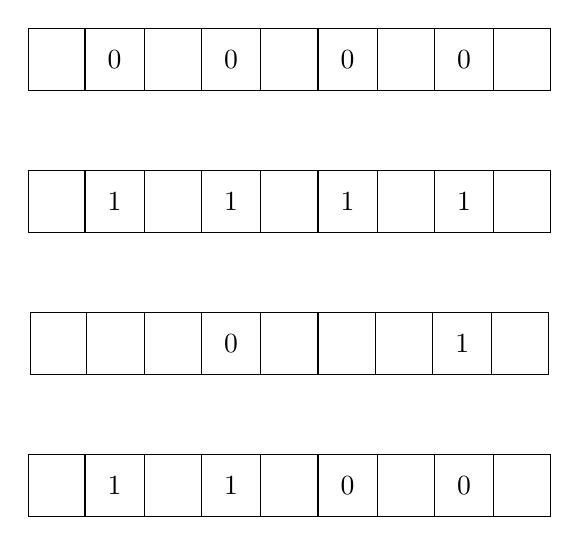
\begin{tikzpicture}[Array/.style = {rectangle split, rectangle split parts = #1, rectangle split horizontal,
    inner sep = 8pt, anchor = center}]
    % even bit: all 0
    \node[Array = {9}, draw] (all0) 
    {\nodepart{two}0\nodepart{three}\nodepart{four}0\nodepart{five}\nodepart{six}0\nodepart{seven}\nodepart{eight}0\nodepart{nine}};

    % even bit: all 1
    \node[Array = {9}, draw, below = of all0] (all1) 
    {\nodepart{two}1\nodepart{three}\nodepart{four}1\nodepart{five}\nodepart{six}1\nodepart{seven}\nodepart{eight}1\nodepart{nine}};

    % even bit: 0 .. 1
    \node[Array = {9}, draw, below = of all1] (01) 
    {\nodepart{two}\nodepart{three}\nodepart{four}0\nodepart{five}\nodepart{six}\nodepart{seven}\nodepart{eight}1\nodepart{nine}};

    % even bit: 1 .. 1 0 .. 0
    \node[Array = {9}, draw, below = of 01] (10) 
    {\nodepart{two}1\nodepart{three}\nodepart{four}1\nodepart{five}\nodepart{six}0\nodepart{seven}\nodepart{eight}0\nodepart{nine}};
\end{tikzpicture}
\end{document}
